\subsection{Encoding Functions in Process Calculi}
\label{sec:blue}
Process Calculi are used to describe the structure and behaviour of concurrent processes.  As a basis for the design of programming languages, a calculus should be able to encode canonical calculations with functions.  Encoding the $\lambda$-calculus, the canonical form of functional programming, to a processes calculus could be done either indirectly or directly.  

\subsubsection{Indirect Encoding}
In \cite{function_as_process}, Milner gave translation rules from both the lazy $\lambda$-calculus and the call-by-value $\lambda$-calculus to his $\pi$-calculus.  Based on this work, in an higher-order $\pi$-calculus, functions could be encoded into processes and then passed around the network as a value.  Later, Sangiorgi pointed out that the higher-order approach is unnecessary since the plain $\pi$-calculus could simulate this higher-order feature by passing a name that points to the encoding process\cite{HOPI}.

The main drawback of the two indirect encoding approaches is its inefficiency in translation and reduction.  Indirect encoding will yield a mass of intermediate variables.  Moreover, without a direct representation for functions, complex substitutions of variables for functions are unavoidable during reductions.

\subsubsection{The Blue Calculus: Encoding Functions in a Direct Style}
Boudol's blue calculus, $\pi^*$, is a direct extension of both the $\lambda$-calculus and the $\pi$-calculus.  In fact, Boudol defined two calculi in \cite{Blue}: a name-passing $\lambda$-calculus ($\lambda^*$) and an extended $\pi$-calculus without summation and matching ($\pi^*$).  The $\lambda^*$-calculus has $\lambda$-style syntax and $\pi$-style reduction relation (Table \ref{lambda_star}).  It is used as an intermediate language when translating $\lambda$-terms to $\pi^*$-terms.  The $\pi^*$-calculus contains primitives from both the $\lambda^*$-calculus and the $\pi$-calculus so that the translation from both languages is straightforward.

\begin{table} [h]
  \begin{center}
  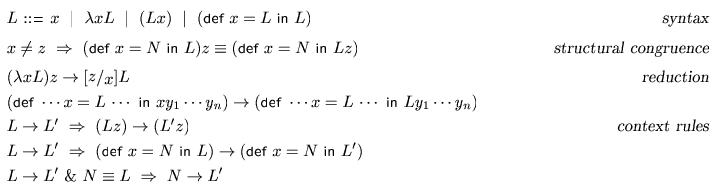
\includegraphics[scale=0.5]{lambda_star.png}
  \end{center}
  \caption{The $\lambda ^*$-calculus}
  \label{lambda_star}
\end{table}

The $\lambda^*$-calculus differs from the $\lambda$-calculus in two aspects:
\begin{inparaenum}[(i)]
  \item The argument ($N$) in an application ($M N$) must be a variable.
  \item A convenient notation for name declaration, $def\ x\ =\ N\ in\ M$, is allowed.
\end{inparaenum}
It is important to note that the $\lambda^*$-calculus only contains the call-by-name evaluation.  This simplifies subsequent studies on relationship between the $\lambda$-calculus and other calculi.  Translations from $\lambda$ to $\lambda^*$ is similar to Launchbury's encoding in \cite{Launchbury93anatural}:

\begin{center}
  \begin{tabular}{ r c l  c}
$x^*$&=&$x$&\\
$(\lambda xM)^*$&=&$\lambda xM^*$&\\
$(M N)^*$&=&$(def\ v = N^*\ in\ (M^*v))$&($v$ fresh)\\
  \end{tabular}
\end{center}

As mentioned earlier, both the $\lambda^*$-calculus and the $\pi$-calculus (without summation and matching) could be translated to the  $\pi^*$-calculus (see Table \ref{trans_blue}).  In addition, a CPS \footnote{continuation passing style} transform from the $\pi^*$-calculus to the $\pi$-calculus is given in \cite{Blue} as well.  Lastly, Silvano Dal-zilio \cite{Dal-Zilio97implicitpolymorphic} proposed a implicit polymorphic type sytem for the $\pi^*$-calculus as an improvement of the original simple type system in \cite{Blue}.

\begin{table}[h]
  \begin{center}
  \begin{tabular}{ l r c l r}
syntax:\\
&$P$&::=& $A\ |\ D\ |\ (P\ |\ P)\ |\ (\nu x)P$&processes\\
&$A$&::=& $u\ |\ (\lambda u)P\ |\ (Pu)$&agents\\
&$D$&::=& $\langle u\ =\ P\rangle\ |\ \langle u\ \Leftarrow P\rangle$& declarations\\
structural equivalence:\\
&$(P\ |\ Q)$&$\equiv$&$(Q\ |\ P)$&commutativity\\
&$((P\ |\ Q)\ |\ R)$&$\equiv$&$(P\ |\ (Q\ |\ R))$&associativity\\
&$((\nu u)P\ |\ Q)$&$\equiv$&$(\nu v)(P\ |\ Q)\ \ (u\ is\ not \ free\ in\ Q)$&scope migration\\
&$(P\ |\ Q)u$&$\equiv$&$(Pu\ |\ Qu)$&distributivity\\
&$((\nu u)P)v$&$\equiv$&$(\nu u)(Pv)\ \ (u\ \neq\ v)$&\\
&$Du$&$\equiv$&$D$&\\
&$\langle u\ =\ P\rangle$&$\equiv$&$\langle u\ \Leftarrow\  (P\ |\ \langle u\ =\ P\rangle )\rangle$&duplication\\
reduction:\\
&$((\nu u)P)v$&$\rightarrow$&$[v/u]P$&$\beta$\\
&$(u\ |\ \langle u\ \Leftarrow\ P \rangle)$&$\rightarrow$&$P$&resource fetching
  \end{tabular}
  \end{center}
  \caption{The $\pi^*$-Calculus}
  \label{blue}
\end{table}

\begin{table}[h]
  \begin{center}
  \begin{tabular}{ r c l r c l}
$[x]u$&=&$\overline{x}u$&$[\overline{u}v_1\cdots v_k]$&=&$uv_1\cdots v_k$\\
$[\lambda xL]u$&=&$u(x,v)[L]v$&$[u(v_1, \cdots ,v_k)P]$&=&$\langle u\ \Leftarrow\ (\lambda v_1 \cdots v_k)[P]\rangle$\\
$[Lx]u$&=&$(\nu x)([L]v\ | \ \overline{v}xu)$&$[!u(v_1, \cdots ,v_k)P]$&=&$\langle u\ =\ (\lambda v_1 \cdots v_k)[P]\rangle$\\
$[def\ x\ =\ N\ in\ L]u$&=&$(vx)([L]u\ |\ !x(v)[N]v)$&$[P\ |\ Q]$&=&$([P]\ |\ [Q])$\\
&&&$[(\nu u)P]$&=&$(\nu u)[P]$
  \end{tabular}
  \end{center}
  \caption{Translation from $\lambda^*$-calculus and $\pi$-calculus to $\pi^*$-calculus}
  \label{trans_blue}
\end{table}
